% !TEX encoding = UTF-8 Unicode
% !TEX TS-program = pdflatex

%%%%%%% La riga soprastante serve per configurare gli editor
%%%%%%% TeXShop, TeXworks e TeXstudio per gestire questo file
%%%%%%% con la codifica UFF-8.
%%%%%%% Se si vuole usare un'altra codifica si veda sotto.
%%%%%%%

%%%%%%%  Esempio con molte opzioni
%%%%%%% Le opzioni nella forma "chiave=valore" sono definite
%%%%%%% perché la classe dalla versione 6.1.00 usa il pacchetto
%%%%%%% xkeyval. Vedere sulla documentazione in inglese o
%%%%%%% in italiano quali chiavi accettano valori.

%%%%%%% L'opzione per il corpo accetta qualsiasi valore, anche fratto
%%%%%%% (per esempio: corpo=11.5pt) e va sempre scritto con una
%%%%%%% unità di misura. L'utente è pregato di non esagerare con
%%%%%%% corpi normali minori di 9.5pt o maggiori di 13pt.
%%%%%%%
%%%%%%% Le opzioni per inputenc e fontenc vanno per prime.
%%%%%%% Vengono ignorate se NON si compone con pdfLaTeX. Ma
%%%%%%% questo è un esempio per pdfLaTeX.
%%%%%%%

\documentclass[%
    corpo=12pt,
    twoside,
    stile=classica,   
% 	oldstyle,
%   autoretitolo,
    tipotesi=magistrale,
    evenboxes,
    english,
%   cucitura=7mm,
	numerazioneromana,
]{toptesi}
%%%%%%%%%%%%%%%%%%%%%%%%%%%%%%%%%%%%%%%%%%%%%%%%%%%%
%%%%%% Per la codifica d'entratasi può scegliere quella che si vuole,
%%%%%% ma si consiglia di preferire utf8; in ogni caso non scegliere
%%%%%% codifiche specifiche del sistema operativo.

\usepackage[utf8]{inputenc}% codifica d'entrata
\usepackage[T1]{fontenc}%    codifica dei font
\usepackage{lmodern}%        scelta dei font

% Vedere la documentazione toptesi-it.pdf per le
% attenzioni che bisogna usare al fine di ottenere un file
% veramente conforme alle norme per l'archiviabilità.


\usepackage[hidelinks]{hyperref}

\hypersetup{%
	pdfauthor={Gabriele Degola},
    pdfpagemode={UseOutlines},
    bookmarksopen,
    pdfnewwindow=true,
    pdfstartview={FitH}
  }
%
%%%%%%% Esempio di composizione di tesi di laurea con PDFLATEX 
%
\usepackage{csquotes}
\usepackage{lipsum}
\usepackage{subcaption}
\usepackage{biblatex}
\addbibresource{references.bib}
\usepackage[acronym]{glossaries}
\usepackage{tabularx}
%

\makeglossaries
\newacronym{ai}{AI}{artificial intelligence}
\newacronym{ilsvrc}{ILSVRC}{ImageNet Large Scale Visual Recognition Challenge}
\newacronym{cnn}{CNN}{Convolutional Neural Network}
\newacronym{gan}{GAN}{Generative Adversarial Network}
\newacronym{svm}{SVM}{Support Vector Machines}
\newacronym{ide}{IDE}{Integrated Development Environment}
\newacronym{iou}{IoU}{Intersection over Union}
\newacronym{roc}{ROC}{Receiver Operating Characteristic}
\newacronym{auc}{AUC}{Area Under the Curve}
\newacronym{ap}{AP}{Average Precision}
\newacronym{map}{mAP}{mean Average Precision}
\newacronym{json}{JSON}{JavaScript Object Notation}
\newacronym{xml}{XML}{Extensible Markup Language}
\newacronym{voc}{VOC}{Visual Object Classes}
\newacronym{kitti}{KITTI}{Karlsruhe Institute of Technology and Toyota Technological Institute}
\newacronym{rcnn}{R-CNN}{region-based Convolutional Neural Network}
\newacronym[firstplural=Regions of Interest (RoIs)]{roi}{RoI}{Region of Interest}
\newacronym{rpn}{RPN}{Region Proposal Network}
\newacronym{fpn}{FPN}{Feature Pyramid Network}
\newacronym{ssd}{SSD}{Single Shot Detector}
\newacronym{yolo}{YOLO}{You Only Look Once}
\newacronym{adda}{ADDA}{Adversarial Discriminative Domain Adaptation}
\newacronym{dann}{DANN}{Domain Adversarial Neural Network}
\newacronym{coco}{COCO}{Common Objects in Context}
\newacronym[firstplural=GPUs]{gpu}{GPU}{Graphics Processing Unit}
\newacronym{cpu}{CPU}{Central Processing Unit}
\newacronym{mlp}{MLP}{multi-layer perceptron}

\glsdisablehyper

%%%%%%% Definizioni locali
\newtheorem{osservazione}{Osservazione}% Standard LaTeX
\ExtendCaptions{english}{Abstract}{Acknowledgements}

\begin{document}
\english
%%%%%%% Questi comandi è meglio metterli dentro l'ambiente
%%%%%%% ThesisTitlePage con o senza asterisco, oppure in un file di
%%%%%%% configurazione personale. Si veda la documentazione
%%%%%%% inglese o italiana.
%%%%%%% Comunque i presenti comandi servono per comporre la
%%%%%%% tesi con i moduli di estensione standard del pacchetto
%%%%%%% TOPtesi.

\begin{ThesisTitlePage}*
\ateneo{Politecnico di Torino}% nome generico dell'Universita'
%\nomeateneo{Weiss Turm}% eventuale nome proprio dell'universita'
\logosede[4.5cm]{logopolito}% logo dell'universita'
\FacoltaDi{DIPARTIMENTO DI\space}% Etichetta della facolta'
\facolta{AUTOMATICA E INFORMATICA}% facolta'
%\Materia{Remote sensing}
\titolo{Domain Adaptation for Object Detection}% 
%\sottotitolo{A data augmentation approach}% 
\CorsoDiLaureaIn{Master Degree in\space}
\corsodilaurea{Data Science and Engineering}% per la laurea
\TesiDiLaurea{Master Thesis}
\def\Candidato{Candidate}
\candidato{Gabriele \textsc{Degola}}% per tutti i percorsi 
\AdvisorName{Supervisor}
\relatore{prof. Paolo Garza}% per la laurea e/o il dottorato
%\tutoreaziendale{Valérian Gonnot}
%\NomeTutoreAziendale{Company advisor\\Neovision}

\sedutadilaurea{\textsc{Anno~accademico} 2021-2022}% per la laurea magistrale
\end{ThesisTitlePage}

%\pagenumbering{roman}

\sommario



% \paginavuota % funziona anche senza specificare l'opzione classica

\ringraziamenti



%\tablespagetrue\figurespagetrue % normalmente questa riga non serve ed e' commentata
\indici

\mainmatter
\english
%\pagenumbering{arabic}

\phantomsection
\chapter*{Introduction}
\addcontentsline{toc}{chapter}{Introduction}

\chapter{Problem definition}

\section{Object detection}\label{sec:detection}
Object detection methods are able to recognize the objects represented in an image and to highlight their position, returning the associated bounding boxes, rectangular boxes which contain an object. The bounding box format depends on the model and on the dataset. Typically, they are determined by the \textit{x} and \textit{y} coordinates of the upper-left corner
%, as in \acrshort{coco} (\ref{sec:coco}),
or of the center
%, as in \acrshort{yolo} (\ref{sec:yolo}),
and by the bounding box width and height.

\begin{figure}[ht]
	\centering
	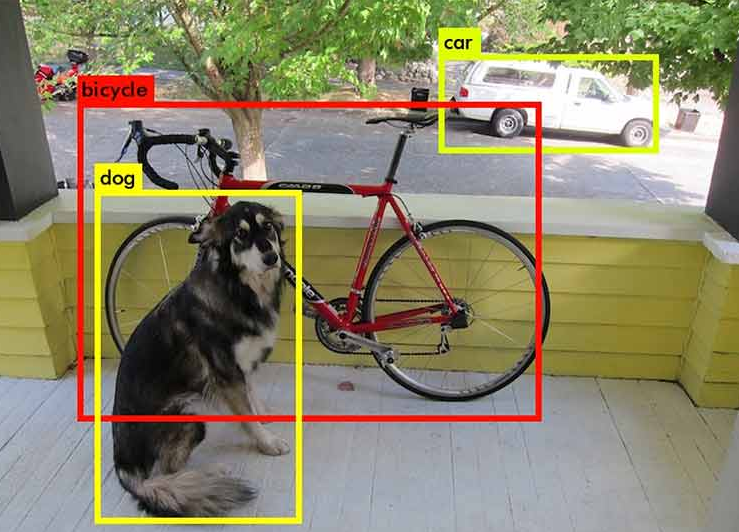
\includegraphics[width=.5\textwidth]{imgs/yolo_detection.png}
	\caption{An example of object detection\cite{redmon2016look}}
\end{figure}

Object detection is a fundamental task in modern computer vision, with applications such as autonomous driving, robot vision and human-computer interaction.

\subsection{Existing methods}\label{sec:detectors}
An object detection task can be seen as a combination of two main steps: finding image regions that may contain objects, and then independently classifying the objects in those regions. Before deep learning, this was achieved using a sliding-window approach, where an image classifier was applied to different areas of the image and only the predictions with the highest probability were retained. Nowadays, two main families of object detectors can be identified.

\subsubsection{Two stage object detectors}
% TODO: spiegare meglio
As said, the most commonly used models for object detection are based on a two-stage approach and belong to the family of \glspl{rcnn}. In basic \acrshort{rcnn}\cite{girshick2014rich}, a manageable number of possible \glspl{roi} are extracted from an image. A \gls{cnn} is then evaluated independently on each \acrshort{roi} to extract features that are fed into a \gls{svm}
%to classify the presence of an object in that region and the bounding box location.
to determine if an object is present in this bounding box (classification task) as well as its location to match that of the object (regression task).
Fast \acrshort{rcnn}\cite{girshick2015fast} and Faster \acrshort{rcnn}\cite{ren2016faster} improved the region selection algorithm, analysing only interesting \glspl{roi} and exponentially reducing the inference time. Because of its good performances and speed, Faster \acrshort{rcnn} is widely used for benchmarking and as base for several derived works.


The main contribution of Faster \acrshort{rcnn} is the introduction of a \gls{rpn}, which integrate some convolutional layers of the image classifier into the region proposal phase. That allows the network to be trained in an end-to-end fashion.

\begin{figure}[ht]
	\centering
	\subcaptionbox{Description of \acrshort{rcnn}\cite{girshick2014rich}}{
		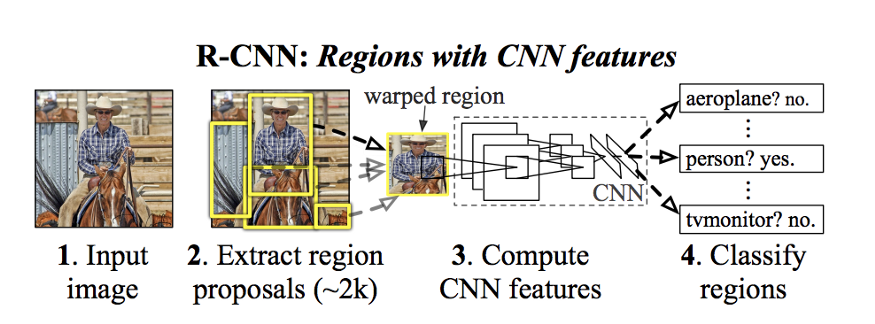
\includegraphics[width=.6\linewidth]{imgs/rcnn.png}
	}
	\subcaptionbox{Description of Faster \acrshort{rcnn}\cite{ren2016faster}}{
		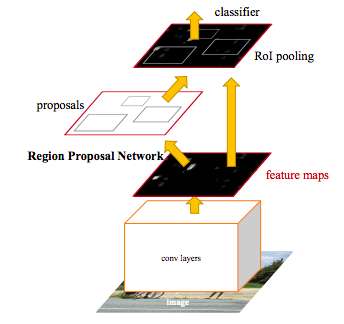
\includegraphics[width=.3\linewidth]{imgs/fasterrcnn.png}
	}
	\caption{Architecture of two stage object detectors}
	\label{fig:architectures}
\end{figure}

\subsubsection{One stage object detectors}
Differently from two stage detectors, one stage object detectors skip the region proposal step and focus on predicting object regions and classes together. This leads to faster predictions with respect to two stage models, making them suitable for real-time applications at the cost of lower prediction quality. The pioneer work for one stage object detection is OverFeat\cite{sermanet2014overfeat}, published in 2014. Here, the last classification layers of a standard \gls{cnn} are replaced by a regression network for each class, in order to predict the object bounding boxes.

\paragraph{YOLO}\label{sec:yolo}
The \acrfull{yolo} model\cite{redmon2016look} uses pretrained \gls{cnn} for classification and splits each image in cells. If the center of an object falls into a cell, that cell is responsible for detection and should predict the bounding box locations, a confidence score and a class probability for the detected objects. A specific loss function is used to efficiently learn at the same time to predict bounding boxes and object classes.

\paragraph{SSD}
\acrfull{ssd}\cite{Liu_2016} adds several convolutional layers of decreasing sizes, in order to build a \textit{pyramid representation} of the images and efficiently detect object of different sizes, at each pyramidal layer. Instead of splitting images in cells, anchor boxes are used for faster detection.

\begin{figure}
	\centering
	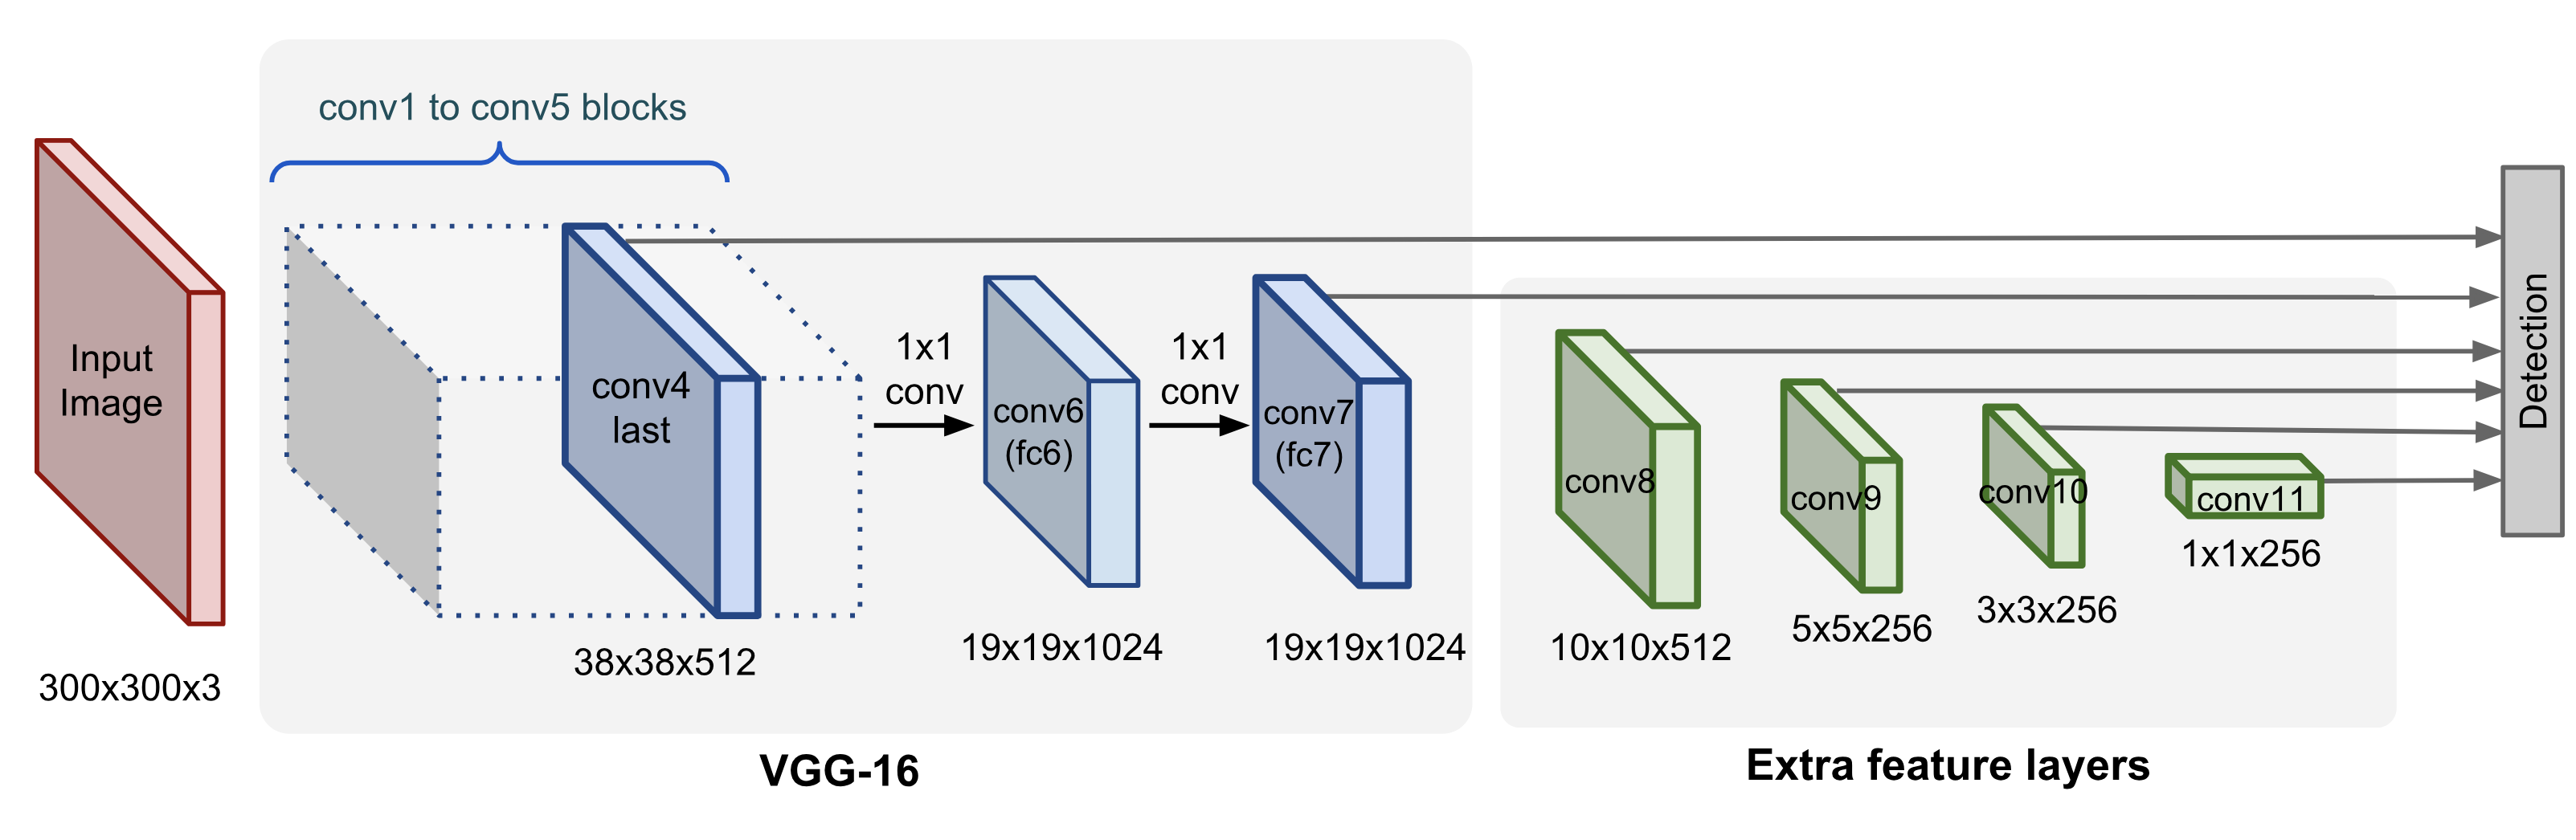
\includegraphics[width=.7\linewidth]{imgs/SSD-architecture.png}
	\caption{\acrshort{ssd}'s pyramid architecture\cite{objdetpart4}}
	\label{fig:ssd}
\end{figure}

After their proposal, both \gls{yolo} and \gls{ssd} have been extensively studied and improved by the community. The last versions of the two families are architecturally close and work in very similar ways.

\paragraph{RetinaNet}
The main improvements of RetinaNet\cite{lin2018focal} over previous one stage detection model are the use of \textit{\acrfull{fpn}} as part of the backbone and of \textit{focal loss}, which helps to approach the results of two-stage detectors.

\begin{figure}[ht!]
	\centering
	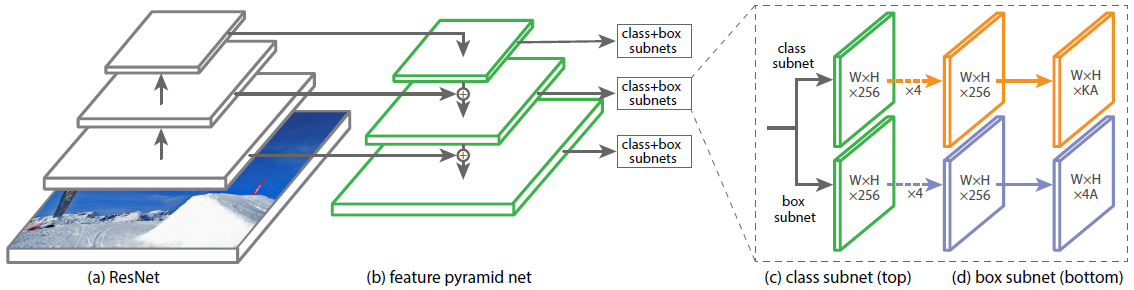
\includegraphics[width=0.8\linewidth]{imgs/retinanet.png}
	\caption{RetinaNet architecture\cite{lin2018focal}}
	\label{fig:retinanet}
\end{figure}

\subparagraph{Feature Pyramid Network}
\glspl{fpn}\cite{lin2017feature} adopt and improve the same approach as \acrshort{ssd}'s pyramid layers. They are composed by a sequence of pyramid levels which correspond to network stages. Each stage is composed by multiple convolutional layers of the same size, divided by two at consecutive stages. In addition to standard feedforward, different stages are linked by a top-down pathway in the opposite direction and lateral connections. This allows the network to construct a rich and multi-scale feature pyramid for each input image.

After their proposal in the context of single-stage detectors, \glspl{fpn} have also been used as part of the backbone of two-stage detectors, to improve their performance.

\subparagraph{Focal loss}
One of the main obstacles for the training of other object detection models is the large imbalance between background and foreground examples, which drives the model to focus on irrelevant background regions. Loss functions are one of the fundamental bricks of deep learning: they are mathematical functions that map an event or the values of one or more variables to a real number, which intuitively represents a certain cost associated with these values. Therefore, each training of deep neural networks aims at minimizing or maximizing one or more loss functions that depend on the problem. In this case, a specific loss function can be used to encourage the network to focus on important regions in the images.

\bigskip
The focal loss, introduced by RetinaNet, is based on the \textit{cross entropy} loss. For binary classification, the cross entropy loss is widely used and defined as:
\begin{center}
	$CE(p,y) = \begin{cases}
		-\log(p) & \text{if $y$ = 1}\\
		-\log(1-p) & \text{otherwise.}
	\end{cases}$
\end{center}
where $y\in \{\pm 1\}$ is the ground truth class and $p\in\left[0,1\right]$ is the model's probability for class $1$. Defining $p_t$ as:
\begin{center}
	$p_t = \begin{cases}
		p & \text{if $y$ = 1}\\
		1-p & \text{otherwise.}
	\end{cases}$
\end{center}
cross entropy can be written as $CE(p,y) = CE(p_t) = -\log(p_t)$.

\bigskip
A balanced version of the cross entropy loss is sometimes used to deal with class imbalance. A numeric factor $\alpha\in\left[0,1\right]$ can be introduced for class $1$, with value $1-\alpha$ for class $-1$. $\alpha_t$ is defined analogously to $p_t$. Therefore, the balanced cross entropy is written as:
\begin{center}
	$CE(p,y) = -\alpha_t\log(p_t)$.
\end{center}

\bigskip
With cross entropy, also easily classified example ($p$ close to $1$ if $y=1$, to $0$ otherwise) produce a non-negligible value for the loss. In focal loss, an additional modulating factor $\left(1-p_t\right)^\gamma$ is added, with tunable focusing parameter $\gamma$. Focal loss is therefore defines as:
\begin{center}
	$FL(p_t) = -\left(1-p_t\right)^\gamma \log(p_t)$
\end{center}
The contribution of easy detections to the overall loss is more or less important depending on the value of $\gamma$. With a high $\gamma$, well detected objects provide a very little contribution to the total loss.

Considering the strong imbalance between the foreground ($y=1$) and background ($y=-1$) classes, the focal loss balanced by the $\alpha_t$ parameter as previously defined is used in RetinaNet:
\begin{center}
	$FL(p_t) = -\alpha_t\left(1-p_t\right)^\gamma \log(p_t)$.
\end{center}

\subsection{Basic components}
\subsubsection{Metrics}
Algorithm evaluation is a fundamental part of machine learning projects and can be performed in different ways, depending on the task and objective. Object detection is a more complex task than traditional classification: a non-fixed number of objects can be present in the same image and the detection model has to accurately predict their position and class. For this reason, dedicated metrics must be introduced and defined.

\paragraph{Precision and recall}
First, the following concepts must be defined in the context of object detection:
\begin{itemize}
	\item \textbf{True positive} (TP): object correctly detected;
	\item \textbf{False positive} (FP): incorrect detection, an object is detected but is not actually present in the bounding box or only partly;
	\item \textbf{False negative} (FN): an object present is the image is not detected by the model.
\end{itemize}
The concept of true negative (TN) does not make sense in an object detection context, as the missing detection of a non-present object is not relevant. In fact, this would mean that the model has correctly identified the background as not belonging to any class.

\subparagraph{Precision}
Precision measures how accurate the predictions of the model are, so it returns the percentage or fraction of correct prediction.
\begin{center}
	$precision = \frac{TP}{TP+FP}$
\end{center}

\subparagraph{Recall}
Recall measures the model detection ability, so it returns the percentage or fraction of correctly detected objects.
\begin{center}
	$recall = \frac{TP}{TP+FN}$
\end{center}

\paragraph{Intersection over union}
For each predicted bounding box, the overlapping with the ground truth bounding boxes is computed, in order to classify the prediction as true or false positive. For a couple of bounding boxes, \gls{iou} is computed as:
\begin{center}
	$IoU = \frac{area\ of\ overlap}{area\ of\ union}$
\end{center}
The computed value is then compared to a threshold to classify a prediction as correct or not. Typical values for the threshold are $0.5$, $0.75$ and $0.95$ and that defines how much we want a detection to be precise. Indeed, a detection classified as true positive with a certain threshold may be considered as false positive if a higher value is used.

\paragraph{Mean Average Precision (mAP)}
\gls{roc} curve is a popular concept in machine learning. There, recall (or true positive rate) and false positive rate are plotted at different classification thresholds. The associated \gls{auc} metric considers the area under the \gls{roc} curve to assess the performances of a model.\cite{roc} It ranges from $ 0 $ to $ 1 $, with $ 0 $ meaning the model's predictions are all wrong and $ 1 $ they are all correct. Ideally, the \gls{auc} score is $ 0.5 $ for a model that returns random predictions.

Similarly, the precision-recall curve shows the trade-off between precision and recall for different thresholds\cite{precrecall}. \gls{ap} is defined as the area under the precision-recall curve. A high area under the curve means both high recall and high precision. The definition of \gls{map} depends on the context. If \gls{ap} is independently computed for each class or for different \gls{iou} thresholds, then \gls{map} is the average of \gls{ap}. In other cases, \gls{map} and \gls{ap} can be used interchangeably.


\subsubsection{Datasets}\label{sec:datasets}
Several datasets have been published to evaluate the performances of object detection algorithms for different use cases.

\paragraph{COCO}\label{sec:coco}
\gls{coco} is a large-scale object detection and object segmentation dataset published by Microsoft, containing over 200000 images for 91 classes, annotated with bounding boxes and at pixel level\cite{lin2015microsoft}. It defines its own annotation format as \acrshort{json} files.

\paragraph{PASCAL VOC}
PASCAL \gls{voc} is a classification and object detection dataset, developed for different machine learning competitions between 2005 and 2012\cite{voc}. Annotations are stored in \acrshort{xml} format, with a file for each image in the dataset. Bounding boxes are determined by the $x$ and $y$ coordinates of the upper left and bottom left corners.

\paragraph{CityScapes}
CityScapes is an object segmentation dataset containing 5000 street scenes images from 50 different cities, with the aim of training models for autonomous driving\cite{cordts2016cityscapes}. When used for object detection, bounding boxes can be derived from the tightest rectangles containing the segmentation masks.

\paragraph{KITTI}
The \gls{kitti} dataset\cite{Geiger2013IJRR} contains 7481 images captured in a context similar to CityScapes. Bounding box annotations are stored in plain text, with one file per image.

\paragraph{Sim10k}
Sim10k is a synthetic dataset containing 10000 annotated images for car detection, rendered from the video-game Grand Theft Auto 5, with the objective of training models in a rich virtual world for detection in the real\cite{johnsonroberson2017driving}.

\begin{figure}[ht]
	\centering
	\subcaptionbox{CityScapes\cite{cordts2016cityscapes}}{
		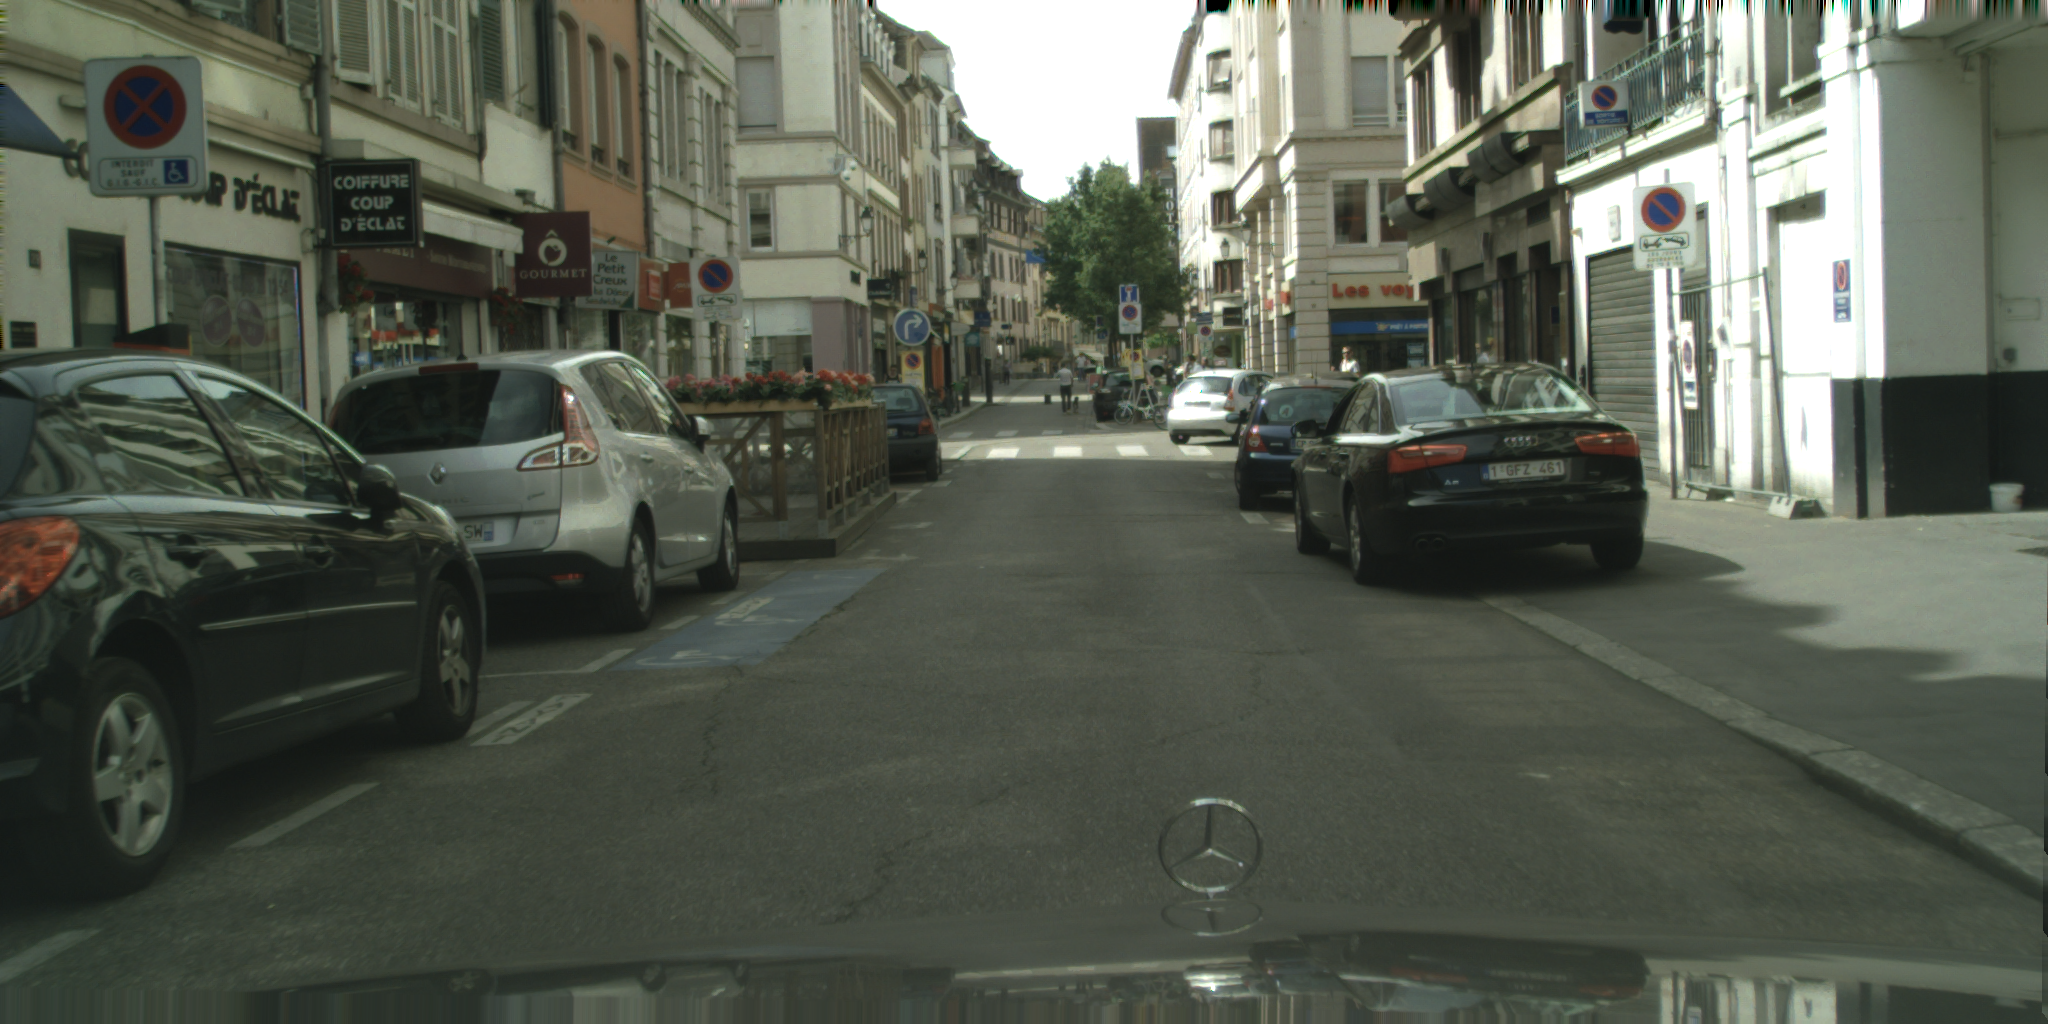
\includegraphics[width=.60\linewidth]{imgs/cityscapes.png}
	}
	\subcaptionbox{\acrshort{kitti}\cite{Geiger2013IJRR}}{
		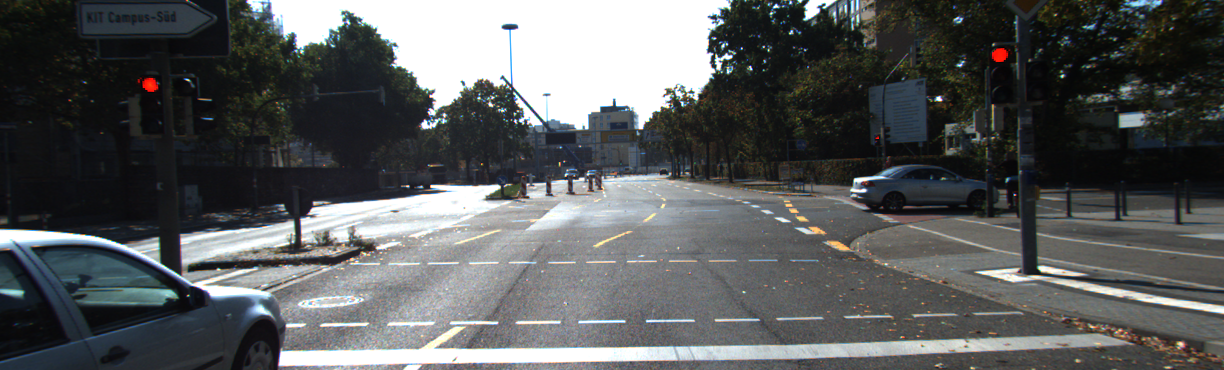
\includegraphics[width=.60\linewidth]{imgs/kitti.png}
	}
	\subcaptionbox{Sim10k\cite{johnsonroberson2017driving}}{
		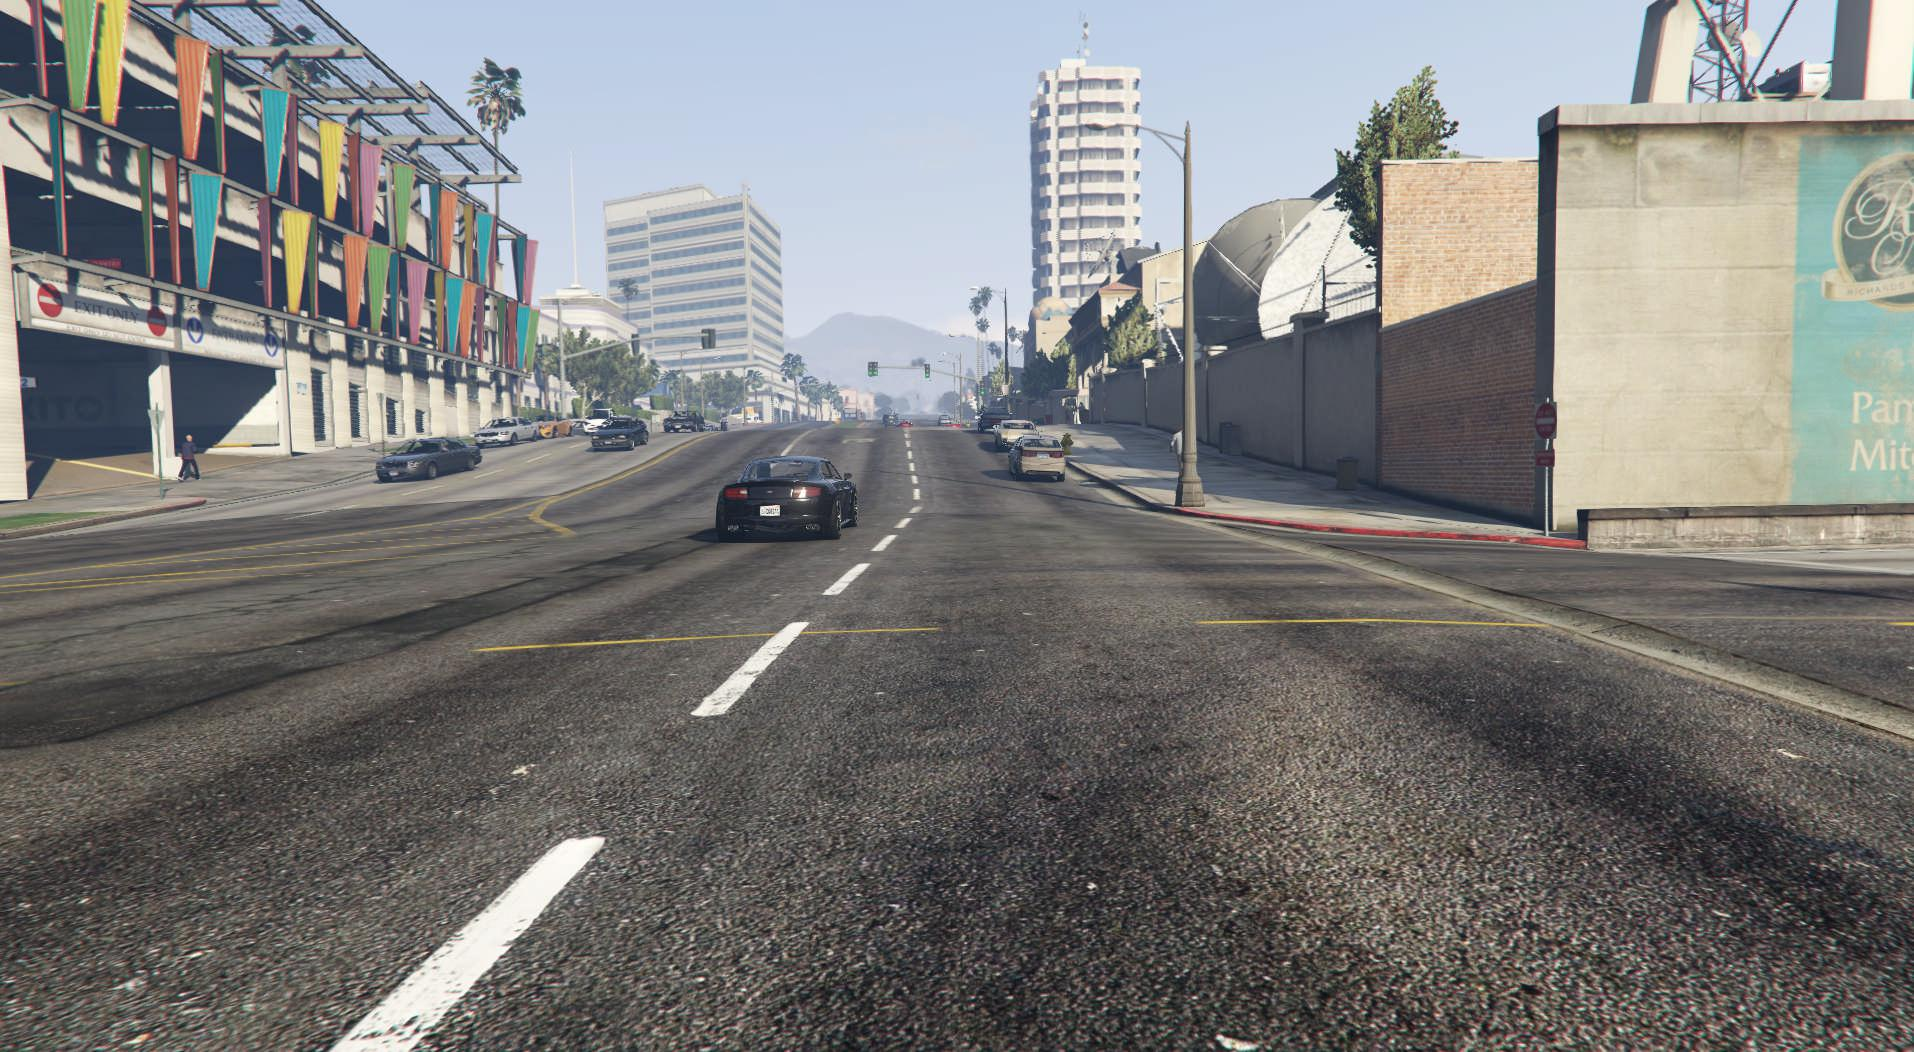
\includegraphics[width=.60\linewidth]{imgs/sim10k.jpg}
	}
	\caption{Examples of different street scenes datasets. It is evident that the appearance of images from different domains varies, even if they contain the same categories of objects.}
	\label{fig:datasets}
\end{figure}

\subsubsection{Anchor boxes}\label{sec:anchor}
In most cases, generating a large number of possible bounding boxes is too cumbersome and leads to inaccurate predictions. If we already know which classes we want to detect, it may be more efficient to define a-priori a set of possible aspect ratios and zoom factors for the bounding boxes. For example, if we are interested in detecting cars wide anchor boxes can be defined at different scales, to identify both near and far objects.

\subsubsection{Non-maximum suppression}
Object detection models usually produce more than one detection for each object, which is not desirable. Non-maximum suppression (NMS) is a method to select one of many overlapping bounding boxes. For a set of overlapping boxes, the one predicted with the highest confidence is selected and all remaining boxes whose \gls{iou} with the chosen bounding box is over a certain threshold are discarded. In this way, only the most probable detection is kept for each object.

\begin{figure}[ht]
	\centering
	\subcaptionbox{Before NMS}{
		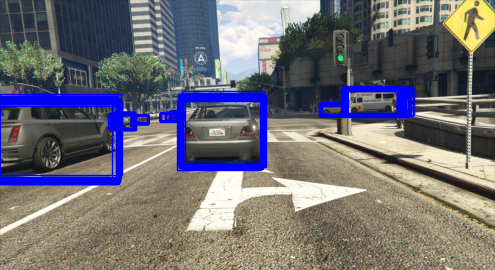
\includegraphics[width=.70\linewidth]{imgs/no_nms.png}
	}
	\subcaptionbox{After NMS}{
		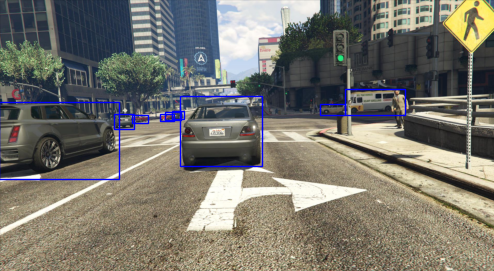
\includegraphics[width=.70\linewidth]{imgs/nms.png}
	}
	\caption{Example of application of non-maximum suppression}
	\label{fig:nms}
\end{figure}


\section{Domain adaptation}

% TODO: add randomization

For most cases, a huge number of annotated images are necessary to train robust and efficient deep learning models. In an industrial context, the process of collecting and annotating data suitable for each specific customer case is often too expensive and time-consuming. In contrast, synthetic data can be generated through various rendering software, even free and open-source, easily and in massive quantities, for simulating the environments in which the models will be applied. However, deep learning models are effective if the training and test data are drawn from the same distribution, so a model trained on simulated data is likely to perform badly on real data. Domain adaptation techniques can be used to transfer knowledge acquired on the \textbf{source domain} (e.g., synthetic data) to the \textbf{target domain} (e.g., real data) without training a new model on the latter. In a domain adaptation setting, the task to be performed on source and target domains and the classes to be predicted remain the same, while the domain differs.

Domain adaptation methods are effective for several computer vision tasks, when dealing with image classification, object detection and semantic segmentation. In addition to the knowledge transfer from synthetic to real images, among other cases they can be used to adapt a model to different cameras, different weather conditions and moments of the day (e.g. from sunny to rainy weather or from day to night) or from infrared to normal images.

Different type of domain adaptation can be identified, based on whether an\-no\-ta\-tions are available or not for the target domain:

\begin{itemize}
	\item \textbf{unsupervised domain adaptation}: labeled source data and unlabeled target data are available;
	\item \textbf{semi-supervised domain adaptation}: labeled source data and some labeled target data are available;
	\item \textbf{supervised domain adaptation}: labeled data are available for both domains.
\end{itemize}
Moreover, domain adaptation can be classified as \textbf{homogeneous}, if the domains share the same feature space, or \textbf{heterogeneous}, if features differ.

Domain adaptation is mostly studied in the unsupervised and homogeneous scenario, with one source and one target domain.

\subsection{Domain adaptation methods}
Different approaches to the problem has been proposed in recent years. The most frequent ones are \textit{domain-invariant feature learning} and \textit{domain mapping}.

\subsubsection{Domain-invariant feature learning}
Several methods try to align source and target domains by creating a domain-invariant feature representation at the level of the feature extractor neural network. Intuitively, if a model performs well on domain-invariant features extracted from the source domain, it should generalize to the target domain since the two distributions are aligned. A schema is reported in Figure~\ref{fig:align}.

\begin{figure}[ht]
	\centering
	\subcaptionbox{Training}{
		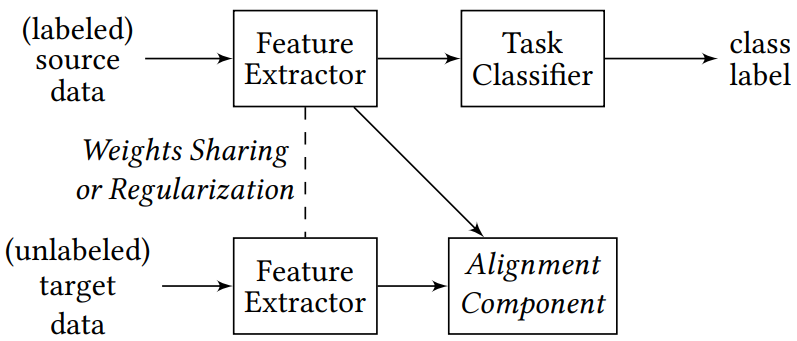
\includegraphics[width=.4\linewidth]{imgs/align_train.png}
	}
	\subcaptionbox{Testing}{
		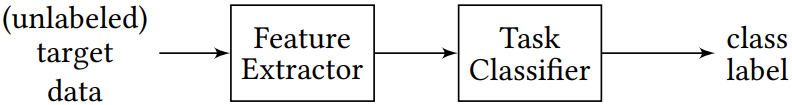
\includegraphics[width=.4\linewidth]{imgs/align_test.png}
	}
	\caption{General schema for domain-invariant feature learning\cite{wilson2020survey}}
	\label{fig:align}
\end{figure}

The methods differ in how they align the domains. An adversarial approach, as in \glspl{gan}, is often used through a domain classifier which outputs whether the features extracted by the \gls{cnn} belong to source or target domain. At the same time, the feature extractor is trained with the aim of fooling the domain classifier, so that it is unable to correctly classify from which domain the feature representation originates. The two networks are trained simultaneously and in an adversarial fashion.

\subsubsection{Domain mapping}
An alternative to creating a domain-invariant feature representation is mapping one domain to the other, making source images similar to the target or vice versa. For example, synthetic images from \textit{Sim10k} can be mapped to the real world, transferring them to the \textit{CityScapes} style. This can be obtained with conditional \glspl{gan} for image-to-image translation that do not take into account the annotations of source images. Therefore, domain adaptation can be accomplished by training a \gls{gan} to map data from source to target and then training a machine learning model on the mapped labeled source images (that now belong to the target domain). At test time, the model is used to make predictions on unlabeled target data. A general schema is reported in figure~\ref{fig:gan}. However, \gls{gan} training is challenging and may incur in several problems such as mode collapse, when a generative network is only capable to produce a limited amount of output images.

\begin{figure}[ht]
	\centering
	\subcaptionbox{Training}{
		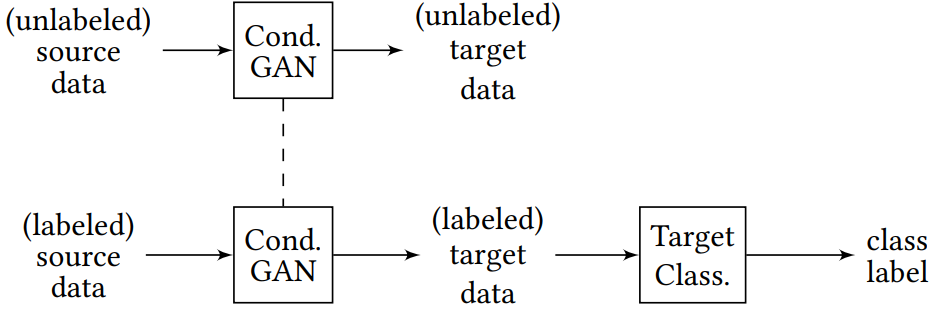
\includegraphics[width=.55\linewidth]{imgs/gan_train.png}
	}
	\subcaptionbox{Testing}{
		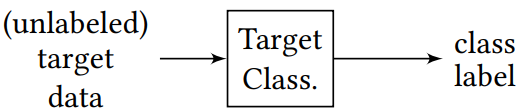
\includegraphics[width=.3\linewidth]{imgs/gan_test.png}
	}
	\caption{General schema for domain mapping\cite{wilson2020survey}}
	\label{fig:gan}
\end{figure}

% TODO: mention enhancing photorelism enhancement

\subsubsection{Previous works}
This section introduces the main methods proposed in the literature for unsupervised domain adaptation in an image classification scenario.

\paragraph{Domain Adversarial Neural Network}\label{sec:dann}
\gls{dann}\cite{ganin2015unsupervised} is a classic method for un\-su\-per\-vi\-sed domain adaptation with the objective of learning domain invariant features. The network is composed of a standard feature extractor, a label predictor and a domain classifier. This work introduces the gradient reversal layer: it leaves input unchanged during the forward step and reverses the gradient during backpropagation, multiplying it by a negative factor. The network is trained adversarially, with the aim of minimizing the label predictor’s loss, while seeking feature mapping parameters that maximize domain classifier loss and domain classifier parameters that minimize its loss. The objective is to align the two data distributions, fooling the domain classifier: when alignment is accomplished, the label predictor is capable of correctly classify an image, whether it is taken from the source or the target domain, while the domain classifier can only return random guesses. A network representation is reported in Figure~\ref{fig:dann}.

\begin{figure}[ht!]
	\centering
	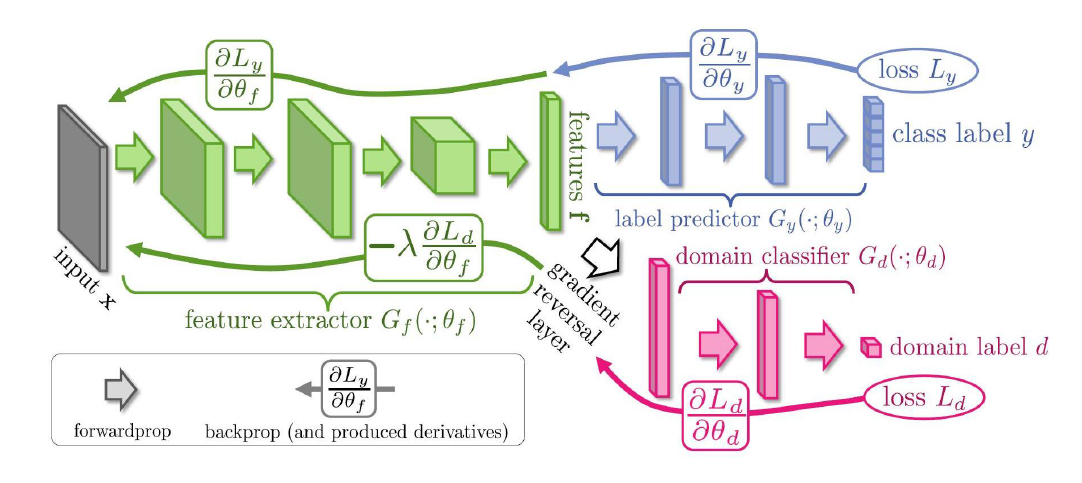
\includegraphics[width=0.8\linewidth]{imgs/dann.png}
	\caption{\gls{dann} architecture\cite{ganin2015unsupervised}}
	\label{fig:dann}
\end{figure}

% TODO: formula dann con gamma, parametri ripresi più avanti

\paragraph{Adversarial Discriminative Domain Adaptation}\label{sec:adda}
\gls{adda}\cite{tzeng2017adversarial} is an adversarial method like \gls{dann}, but is composed by three consecutive phases:
\begin{enumerate}
	\item A \gls{cnn} is trained on labeled source examples in order to learn a feature representation for the source domain that can be successfully identified by a classifier. The source \gls{cnn} is frozen.
	\item Adversarial adaptation is then performed. The objective is to train a target feature extractor in a way that a discriminator which receives features extracted from the two domains cannot predict their domain label, in order to align the domain representations. This is done through \textquotedblleft flipped labels\textquotedblright : the training procedure fools the domain discriminator into believing that the features ex\-trac\-ted from the target domain belong to the source domain instead. As a consequence, the target feature extractor is lead to learn features for the target domain that the domain discriminator could misclassify (as belonging to the source domain).
	\item For inference, target images are mapped to the shared feature space and classified by the source classifier trained at the beginning.
\end{enumerate}
A method overview is reported in Figure~\ref{fig:adda}.

\begin{figure}[ht!]
	\centering
	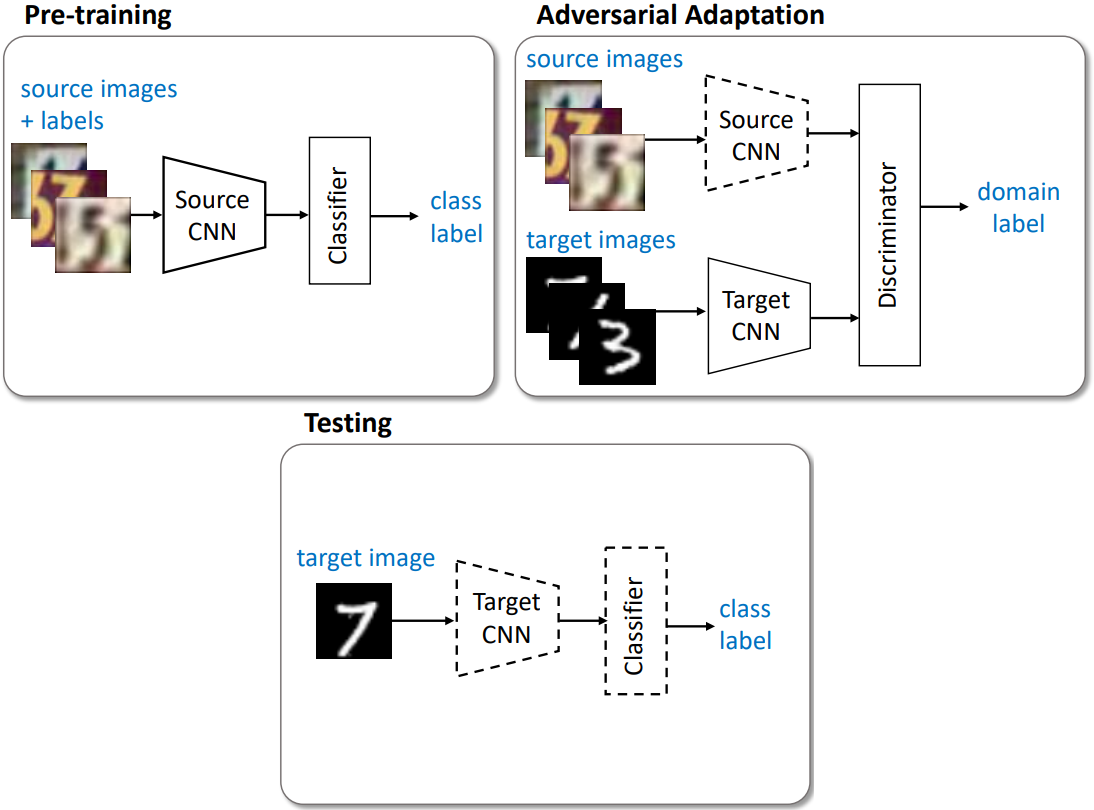
\includegraphics[width=0.9\linewidth]{imgs/adda.png}
	\caption{\acrshort{adda} working schema\cite{tzeng2017adversarial}. The dashed lines indicate the parts of the networks that are frozen after the previous step, while the remaining parameters are learned.}
	\label{fig:adda}
\end{figure}

\iffalse
\paragraph{Asymmetric Tri-Training}
Differently from the previous mentioned methods, asymmetric tri-training\cite{saito2017asymmetric} performs adaptation through pseudo-labelling. Three networks, sharing the same feature extractor, are used. Two of them include a classifiers trained on source labeled images, with the aim of classifying features extracted from target image. If their predictions are coherent and with high confidence, the predicted pseudo-labels are assigned to those images. The third network is then trained with those pseudo-labels. An additional \gls{loss} is used to force a different point of view for the two source classifiers.
\fi

\subsection{Domain adaptation for object detection}
Like classification models, object detectors suffer from domain shifts between different datasets, which can lead to drastic \gls{map} drops and performance degradation. Annotating images for an object detection task is even more expensive and time-consuming than classification, since each image may contain more than one object that needs to be assigned a bounding box and object category. Due to the different nature of the problem, direct translation of domain adaptation methods for classification may not be effective, and ad-hoc methods have been proposed, generally based on existing object detectors.

\subsubsection{Previous works}
\paragraph{Domain Adaptive Faster R-CNN}\label{sec:dafrcnn}
DA Faster \acrshort{rcnn}\cite{chen2018domain} is one of the first works to tackle the problem of cross-domain object detection. It uses a Faster \acrshort{rcnn} as base object detector and the network is trained with adaptation with gradient reversal layers at different levels. Indeed, in an object detection scenario the domain shift can occur at high level, such as image style and illumination, and at low level, such as object appearance and bounding box size. The former is referred to as \textit{image level}, while the latter is defined as \textit{instance level}. An additional loss function, referred as \textit{consistency loss}, is used to enforce consistent prediction from the two domain classifiers.

At inference time, the aligned Faster \gls{rcnn} is normally used.

\paragraph{Strong-Weak Distribution Alignment}
Aligning image level features as in DA Faster \acrshort{rcnn} makes the strong assumption that image components, such as backgrounds and scene layouts, must be similar across domains in addition to object categories. In the case of large domain shifts, that may affect the model performances. Saito \emph{et al.}\cite{saito2019strongweak} propose a weak global alignment (at image level) combined with a strong alignment of local features (such as the texture or the color of the domains), which are most likely to be similar.

For weak alignment between domains, the domain classifier should focus on examples that are hard to classify, so near the boundary between the two distributions. This can be achieved using the focal loss to train the domain classifier, in order to tune the importance to source or target images whose domain is easy to predict.

\paragraph{Progressive Domain Adaptation}
Hsu \emph{et al.}\cite{hsu2019progressive} introduce an intermediate domain between source and target, exploiting a \gls{gan} to map source images in the target domain. Adaptation is performed in two steps, from source to intermediate and then from intermediate to target, in order to introduce a bridge between source and target domains. That helps to reduce the domain shift and simplify the adaptation process, such that an object detection model can be trained on the intermediate domain. In addition, a weight is assigned to generated data, giving more importance to images that are close to the target distribution.

\paragraph{Domain Adaptive RetinaNet}\label{sec:daretinanet}
Recently, Pasqualino \emph{et al.}\cite{pasqualino2020unsupervised} proposed an adaptation approach for the RetinaNet model, but that can be applied to any architecture that includes a \gls{fpn} backbone. Different domain discriminators with different architectures are applied at different levels of the ResNet backbone which is used to construct the feature pyramid, with gradient reversal layers. In this way, extracted features are aligned at different levels in the backbone and the representation derived by the \gls{fpn} is coherent and meaningful.

\paragraph{Image statistics matching}\label{sec:kis}
The method introduced by Abramov \emph{et al.}\cite{abramov2020simple} relies on image transformations at pixel level instead of adversarial techniques or complex architectures. The objective is to transform annotated source images in a way to make them similar to the unlabeled target domain, matching color statistics and histograms. During training, a target image is randomly chosen for each image belonging to the source domain and the mean and covariance of its color channels are aligned and its color histogram are matched accordingly. In this way, a standard detection model can be trained on modified source image with annotations and directly applied on the target domain.

%\blankpagestyle{headings}

%\lipsum[1-2]

\chapter{Method}
\section{Introduction}
The purpose of this Master Thesis is to investigate existing popular methods for domain adaptive object detection.

A common belief is that extremely complex methods are more likely to achieve good performances than simple methods. For neural networks, the trend over the years has been to try making the networks deeper and deeper, which has produced extraordinary results but at the same time lead to several problems in the training procedures. Recently, simple architectures like \textit{MLP-Mixer}\cite{tolstikhin2021mlpmixer} and \textit{Feed-Forward Stack}\cite{melaskyriazi2021need}, composed of \glspl{mlp} only, reached surprisingly good performances in image classification.

A similar question can be raised for the problem of domain adaptation in an object detection scenario: can simple methods perform comparably or even better than the complex ones that are mostly studied in the literature? Indeed, in an industrial context engineers do not often have the time to deeply understand elaborate network architectures, potentially not useful for the problem they are facing, and must consider the trade-off between complexity and expected efficacy. Simple methods that are capable of reaching good performances are researched and can boost their productivity.

For the sake of completeness, the studied methods are implemented and tested on two popular object detection models presented in Section~\ref{sec:detection} when they are compatible with both architectures: Faster \gls{rcnn} and RetinaNet.

\section{Data augmentation}\label{sec:dataaug}
Data augmentation is a widely used technique to ease the training of deep learning models and improve their generalization capability. In a typical application, different transformations are randomly applied on training images, in order to vary their appearance and virtually introduce new data on which a model can learn.

Data augmentations can modify the orientation of the images or operate at pixel level, transforming their color and appearance. Those operations can be geometric, if they geometrically distort the image keeping without modifying its content, or color-based, if they distort color channels without modifying the position of the pixels. Common transformations include horizontal and vertical flip, rotation, translation and color shift. For object detection, the bounding boxes have to be updated coherently with the applied geometric data augmentation.

\begin{figure}[ht!]
	\centering
	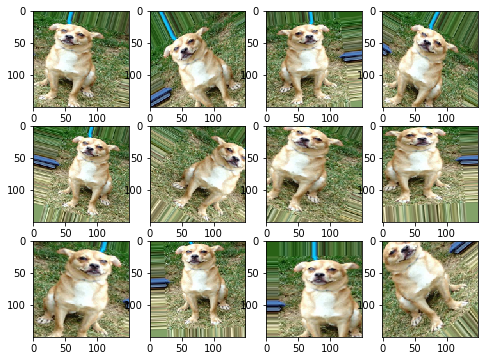
\includegraphics[width=0.7\linewidth]{imgs/augmentation.png}
	\caption{Some examples of data augmentation (image source: \url{http://datahacker.rs/tf-data-augmentation/})}
	\label{fig:augmentation}
\end{figure}

Therefore, data augmentation techniques can extensively alter the image appearance. If a model is trained with high-impact data augmentation on labeled images from a domain, it can potentially achieve good results on a different domain it has never seen. That falls in the case of \textbf{domain randomization}: training images are drawn from a data distribution which is way larger than the original one and the model can learn to generalize to different domains. In some ways, the network is \textquotedblleft overwhelmed\textquotedblright~with different versions of the same images, in order to recognize their contents in different conditions. For domain adaptation, the resulting data distribution can possibly include the target domain or intermediates domains that are closer to the target domain than the source domain.

Most works that investigate domain randomization focus on \textit{sim2real} knowledge transfer and address the problem generating a large variety of synthetic training images. The famous one by Tobin \textit{et al.}\cite{tobin2017domain} defines different randomization parameters that control, inter alia, position, number and type of the objects present in an image, lighting conditions and camera conditions. An interval of values is defined for each parameter and, for generating an image, each parameter is uniformly sampled within its range and used to control the generator. A detection model is then trained on the generated synthetic images and should be able to generalize to real images containing the same kind of objects.

\begin{figure}[ht!]
	\centering
	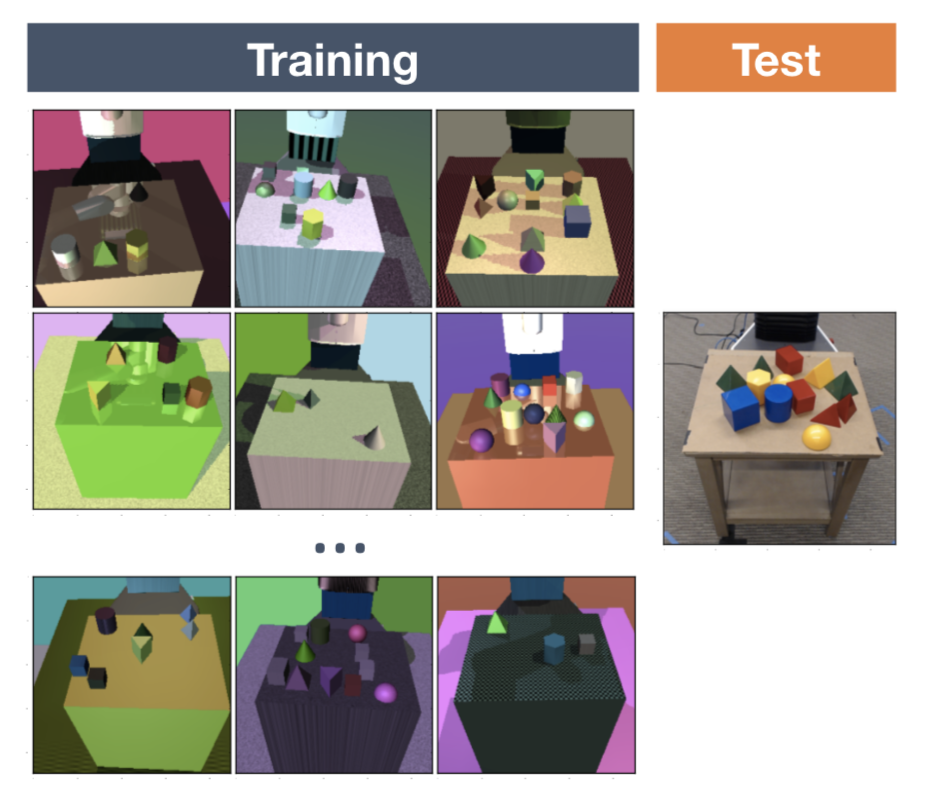
\includegraphics[width=0.6\linewidth]{imgs/randomization.png}
	\caption{Randomization in generating training images\cite{tobin2017domain}}
	\label{fig:randomization}
\end{figure}

In this work, instead, randomization is introduced through the combination of commonly used data augmentation operations, both geometric and color-based:
\begin{itemize}
	\item Horizontal flip: geometric transformation that horizontally mirrors the image.
	\item Rotation: geometric transformation that rotates image and bounding boxes of a degree value sampled from a provided interval.
	\item Translation: geometric transformation that horizontally and vertically translates image and bounding boxes of a number of pixels sampled from a provided interval.
	\item Color jitter: color-level transformation that changes brightness, contrast, saturation and hue of the image. Jitter factors for each properties are sampled from provided intervals.
	\item Solarization: color-level transformation that, for an image, inverts the color of all pixels whose value is above a threshold. The threshold is sampled from a provided interval.
	\item Equalization: color-level transformation that equalizes the color histogram of the image.
\end{itemize}
The operations can be easily implemented and used in most popular deep learning frameworks.

Many other operations are often used for data augmentation, but are not included in the performed experiments due to time constraints and since the possible combinations of the aforementioned operations are already numerous. Examples are shearing, a geometric transformation that deforms the image in parallelogram shape according to horizontal or vertical axis,
%. Each pixel of the image is translated in the same direction, by a magnitude proportional to its distance from the image origin. The amount of shearing is sampled from a provided interval.
and cutout, which randomly masks regions of the training images in order to improve networks' robustness.

\begin{figure}[ht]
	\centering
	\subcaptionbox{Original \textit{Sim10k} image}{
		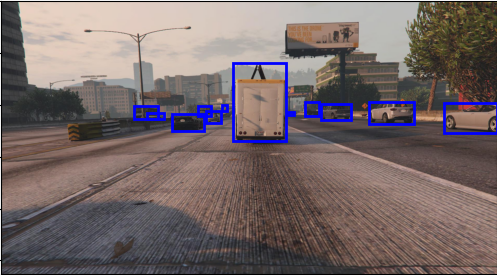
\includegraphics[width=.47\linewidth]{imgs/sim10korig.png}
	}
	\subcaptionbox{\textit{Sim10k} image with augmentations}{
		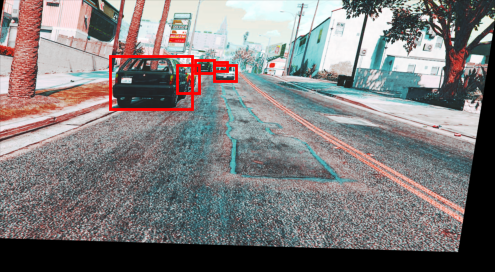
\includegraphics[width=.47\linewidth]{imgs/sim10kaug1.png}
	}
	\subcaptionbox{\textit{Sim10k} image with augmentations}{
		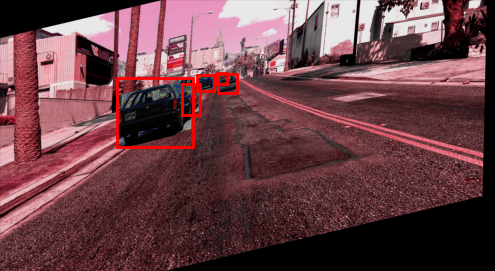
\includegraphics[width=.47\linewidth]{imgs/sim10kaug2.png}
	}
	\subcaptionbox{\textit{Sim10k} image with augmentations}{
		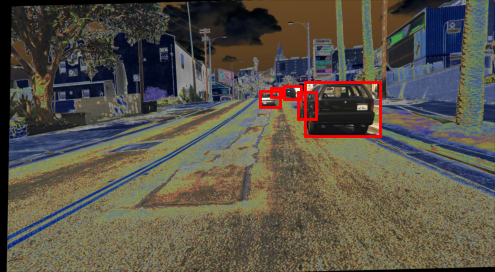
\includegraphics[width=.47\linewidth]{imgs/sim10kaug3.png}
	}
	\caption{Comparison between original and transformed images}
	\label{fig:augs}
\end{figure}

% TODO: autoaugment: problems in geometric operations on small objects (not in boxes anymore) and on background only (image modified, objects covered and not in boxes anymore)

\section{Domain Adaptive Faster R-CNN}
Domain Adaptive Faster \acrshort{rcnn}\cite{chen2018domain}, presented in Section~\ref{sec:dafrcnn}, is without any doubt the most popular method designed to attain successful object detection in different domains. Since its introduction, the paper has been cited hundreds of times and several methods based on it have been proposed. It is therefore a good adaptation method to be used as baseline and for comparison with more advanced architectures.

The training process considers annotated images from the source domain and unlabeled images from the target domain at the same time. Adaptation is performed at two different levels  using the gradient reversal layers presented in Section~\ref{sec:dann}:

\begin{itemize}
	\item Image level: the features extracted by the network backbone are forwarded to a patch-based domain classifier. Such patch classifiers, introduce by Isola \textit{et al.}\cite{isola2018imagetoimage}, divide each feature map of an image into $ N\times N $ patches and classify them independently. For a domain classifier, each patch is classified as extracted from source or target domain. In this way, the importance of the global differences inside images is reduced and the classifier is trained more precisely. Adaptation at this level aims at reducing the global differences such as image style and illumination.
	\item Instance level: the features extracted by the \gls{rpn} are passed to a domain discriminator before being fed to the label classifier and bounding box regressor for the final prediction. That helps reducing differences related to the objects that appear in the images, such as object size, texture and viewpoint.
\end{itemize}
In addition, a consistency regularization is added to encourage similar predictions from the two domain classifiers.

\begin{figure}[ht!]
	\centering
	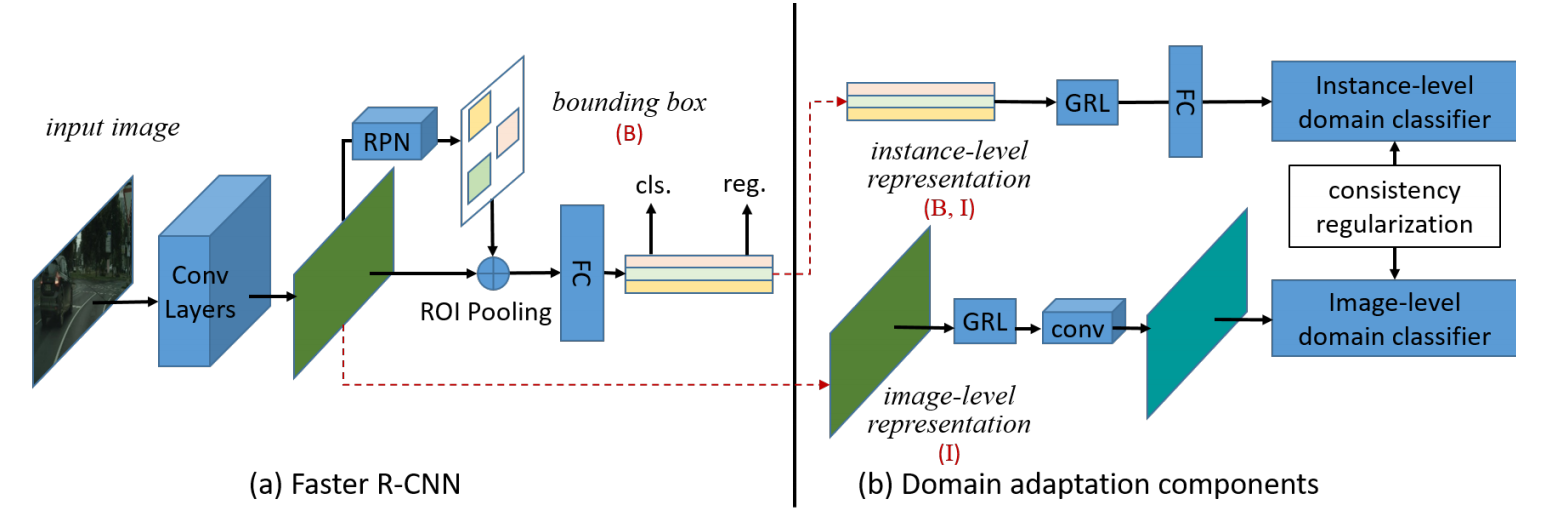
\includegraphics[width=0.9\linewidth]{imgs/dafasterrcnn.png}
	\caption{Overview of the Domain Adaptive Faster \gls{rcnn} model\cite{chen2018domain}}
	\label{fig:dafasterrcnn}
\end{figure}

A training batch is composed by both source and target images and the training procedure is organized as follows:
\begin{itemize}
	\item When the network receives as input labeled images from the source domain, they are used to train both the base Faster \gls{rcnn} and the domain adaptation components.
	\item When the network receives as input unlabeled images from the target domain, they are only used to train the domain adaptation components. Indeed, images are not useful for the base detector as object bounding boxes and classes are not available.
\end{itemize}
For inference, additional components are not considered and the standard Faster \gls{rcnn} with learned weights is used.

\section{Adapting the FPN}
\acrfull{fpn} is a cheap and effective method to increase the performances of a detection model. Nowadays, it is often included in the backbone network of object detectors such as Faster \gls{rcnn} and is one of the fundamental bricks of the RetinaNet model. One of the most popular computer vision frameworks for research, \textit{torchvision} by \textit{PyTorch}\cite{paszke2019pytorch}, only provides pretrained backbones with \gls{fpn} for Faster \gls{rcnn} models. Therefore, using \gls{fpn} for object detection problems is straightforward and highly performing with respect to standard backbones without \glspl{fpn}.

However, \gls{fpn} architecture introduces some problems for adversarial feature alignment on the output of the backbone (as at \textit{image} level in the Domain Adaptive Faster \gls{rcnn} model): backbone layers must be aligned in a way that the extracted feature pyramid representation is logical and coherent. For example, if the alignment is performed on the last backbone layer only, at the end of the training procedure the features extracted from the last layer will be aligned between the domains while the features extracted from the previous may not be so. As \glspl{fpn} construct rich feature representations linking the features extracted from different backbone layers, that would lead to a meaningless feature pyramid. 

\subsection{Implementation on RetinaNet}
Domain Adaptive RetinaNet, introduced in Section~\ref{sec:daretinanet}, takes into account the adversarial domain adaptation for a one-stage object detector with \gls{fpn} backbone. More precisely, in the RetinaNet model the \gls{fpn} uses the features extracted from the last three layers of a ResNet to construct a rich and multi-scale feature pyramid of three levels from a single resolution input image. This representation is then forwarded to two separate fully convolutional sub-networks, in order to predict the probability of the presence of an object in each anchor box and the bounding box locations.

Pasqualino \textit{et al.} perform adaptation through three different domain classifiers with different architectures. They receive the features extracted from the three ResNet layers that are used to build the \gls{fpn} representation. For adversarial alignment, the features are forwarded through gradient reversal layers as in \gls{dann}: the overall network is trained normally but the gradient resulting from the domain classifiers is multiplied by a negative factor, in order to push the ResNet to extract domain invariant features that can be used to accurately detect objects in target images.

%% TODO: caratteristiche dei tre discriminatori

Labeled source images are used to train the whole network, while unlabeled target images only train the three domain classifiers. At test phase, the domain classifiers are plugged off and the adapted RetinaNet is normally used.

\subsection{Implementation on Faster R-CNN}
The addition of a \gls{fpn} component to the backbone of a Faster \gls{rcnn} model improves the detection performances by 3.7 \gls{ap} points on the \gls{coco} dataset\cite{lin2017feature}. The \gls{rpn} receives a rich feature representation at different resolutions and is able to better identify high-quality possible \glspl{roi}. As it can achieve better results than the standard architecture without \gls{fpn} at a negligible price, Faster \gls{rcnn} with \gls{fpn} backbone is commonly used. 

If the base detector includes a \gls{fpn} component, adaptation at image level for the Domain Adaptive Faster \gls{rcnn} method has to be reconsidered. Two possible solutions can be identified in order to align the feature representations between different domains:
\begin{itemize}
	\item Adaptation can be directly performed on features extracted by the \gls{fpn}. Different levels of the feature pyramid can be forwarded, on at a time, to a domain classifier through gradient reversal layer. The resulting domain losses can be summed or averaged across all levels. This way, the objective is to push the ResNet backbone to extract feature representations that can be used to build a feature pyramid which is independent of the domain of each input image.
	\item Similarly to what is done by Pasqualino \textit{et al.}\cite{pasqualino2020unsupervised}, it is possible to directly align the ResNet features that serve as input for the \gls{fpn}: if they are not dependent from the domain, neither the resulting pyramid representation will be. Differently from RetinaNet, the last four ResNet layers are used to build the feature pyramid, so they are forwarded to four different domain classifiers with different architectures, through gradient reversal layers for adversarial alignment.
\end{itemize}
The presence or absence of the \gls{fpn} in the backbone has no impact on adaptation at instance level, as \gls{rpn} returns \glspl{roi} in the same format. If different domain classifiers are used, the consistency regularization loss is independently computed for each ResNet layer between the domain prediction and the prediction at instance level, unique at each iteration. Otherwise, training proceeds as previously described.

\section{Image statistics matching}
As discussed in Section~\ref{sec:dataaug}, data augmentation techniques that significantly modify the appearance of images from a domain extend their data distribution, possibly covering several domains. A model can be trained on transformed images from the source domain without any architectural modification, possibly performing well on images drawn from a target data distribution.

Likewise, domain mapping methods transform images from a source domain in a way that a model can confused them with images from the target domain: they focus on accurate modifications of images rather than upgrading base architectures. That is typically attained with \glspl{gan} for style transfer, but training of adversarial networks is complicated and time-consuming. Instead, the method one introduced by Abramov \textit{et al.}\cite{abramov2020simple} try to \textquotedblleft keep it simple\textquotedblright performing easy but effective operations at image level, with the objective of matching some statistics between source and target images.

More precisely, for each labeled source image an unlabeled target image is randomly selected and two transformation are applied one after the other:
\begin{enumerate}
	\item Feature Distribution Matching: the first transformation transforms the source image in a way that it obtains the color mean and covariance of the target image, while keeping the image content. It works on each pixel through PCA-Whitening with Singular Value Decomposition.
	\item Histogram Matching: the second transformation is often used in image processing. It manipulates the pixels of the source image in order to align its color histograms to the ones of the target image.
\end{enumerate}
A detection model is therefore trained on labeled mapped images that share image statistics of target images. The model can then be directly used for inference on the target domain without any additional operation.

\begin{figure}[ht!]
	\centering
	% 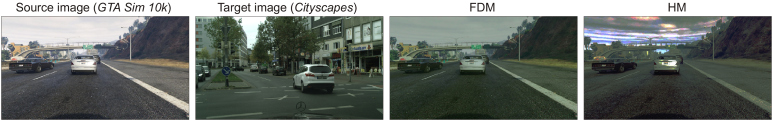
\includegraphics[width=\linewidth]{imgs/kis.jpeg}
	\subcaptionbox{Source image}{
		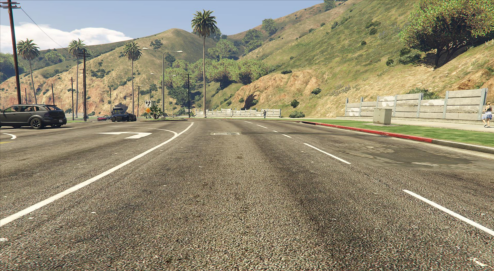
\includegraphics[width=.47\linewidth]{imgs/src.png}
	}
	\subcaptionbox{Target image}{
		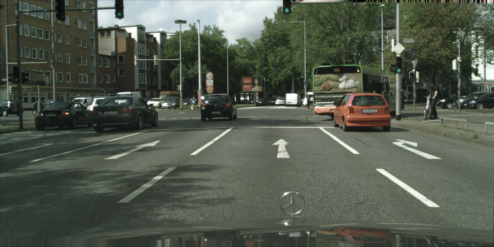
\includegraphics[width=.47\linewidth]{imgs/tgt.png}
	}\\
	\subcaptionbox{Feature Distribution Matching}{
		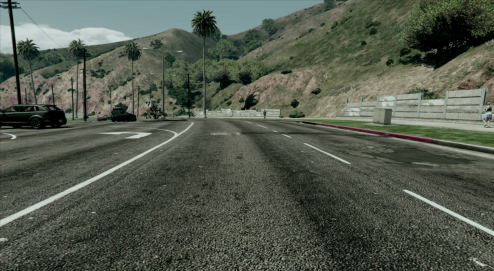
\includegraphics[width=.47\linewidth]{imgs/fdm.png}
	}
	\subcaptionbox{Histogram Matching}{
		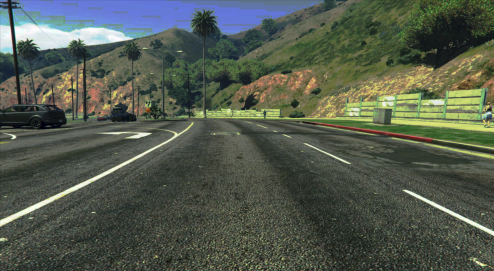
\includegraphics[width=.47\linewidth]{imgs/hm.png}
	}
	\caption{Results obtained through Feature Distribution Matching and Histogram Matching on a sample image. \textit{Sim10k} and \textit{CityScapes} are considered as source and target domains respectively.}
	\label{fig:kis}
\end{figure}

% TODO: trasformazioni a patch

% retinanet + adda ??

\chapter{Experimental results}
\section{Experimental settings}
In this chapter, the results obtained with the tested methods are reported, compared and discussed. For coherence with previous works, \textit{Sim10k} and \textit{CityScapes} are treated as source domain and target domains respectively for training a model to recognize cars in a simulated world for detection in the real. Results are presented in terms of \gls{map} computed at \gls{iou} threshold of $ 0.5 $, separately for the experiments performed with RetinaNet and Faster \gls{rcnn} base detectors. Impact of data augmentation operations in addition to domain adaptation methods is also studied and the transformations employed in each experiment are reported in parentheses.

Parameters and training details were used for all experiments as far as possible. Common settings are:
\begin{itemize}
	\item 15 training epochs;
	\item models pre-trained on \gls{coco};
	\item ResNet-50 backbone;
	\item random data augmentation operators applied with probability $ 0.5 $.
\end{itemize}
The following parameters are used for each data augmentation technique:
\begin{itemize}
	\item random rotation between $ -10 $ and $ 10 $ degrees;
	\item random translation between $ -100 $ and $ 100 $ pixels, independently chosen for the two axis;
	\item brightness, contrast, saturation and hue randomly jittered between $ 0.5 $ and $ 1.5 $, independently chosen for each property;
	\item for solarization, the threshold over which pixels are inverted is randomly chosen between $ 64 $ and $ 192 $ (RGB pixel values going from $ 0 $ to $ 255 $ for each color channel).
\end{itemize}

\section{RetinaNet}
The results obtained with RetinaNet-based methods are reported in Table~\ref{table:retinanet}.

% TODO: maybe separate between randomization and direct adaptation

\begin{table}[ht!]
	\centering
	\begin{tabularx}{\linewidth}{|X|c|}
		\hline
		Method  &   mAP@0.5 \\
		\hline\hline
		Baseline (HFlip + rotation + translation + shearing)      &   39.2   \\
		\hline
		Baseline (HFlip + rotation + translation + shearing + color jitter + solarize + equalize)      &   49.8   \\
		\hline
		Baseline (HFlip + rotation + translation + shearing + box translation + box equalize + equalize)      &   21.0   \\
		\hline
		Baseline (HFlip + box shearing + background color jitter + box equalize)      &   29.1   \\
		\hline
		Baseline (HFlip + rotation + translate y box + equalize)      &   ??.?   \\
		\hline
	\end{tabularx}
	\caption{Extra experiments}
	\label{table:extra}
\end{table}

\begin{table}[ht!]
	\centering
	\begin{tabularx}{\linewidth}{|X|c|}
		\hline
		Method  &   mAP@0.5 \\
		\hline\hline
		Baseline (HFlip)       &   30.4   \\
		\hline
		Baseline (HFlip + rotation + translation)      &   37.6   \\
		\hline
		Baseline (HFlip + rotation + translation + color jitter)      &   49.4   \\
		\hline
		Baseline (HFlip + rotation + translation + color jitter + solarize + equalize)      &   52.7   \\
		\hline
		% TODO: rifare hflip e hflip + rot + transl se c'è tempo
		Image statistics matching (HFlip)  &   48.2    \\
		\hline
		Image statistics matching (HFlip + rotation + translation)  &   52.0    \\
		\hline
		Image statistics matching (HFlip + rotation + translation + color jitter)  &   62.7    \\
		\hline
		DA RetinaNet (HFlip)   &   52.8    \\
		\hline
		DA RetinaNet (HFlip + rotation + translation)   &   54.2    \\
		%54.237
		\hline
		DA RetinaNet (HFlip + rotation + translation + color jitter)   &   54.8    \\
		%54.788
		\hline\hline
		Image statistics matching 2x2 (HFlip) &   45.0    \\
		\hline\hline
		Oracle (HFlip) &   68.7    \\
		\hline
	\end{tabularx}
	\caption{\gls{map} with different domain adaptation method for a RetinaNet model, trained on \textit{Sim10k} and evaluated on \textit{CityScapes}.}
	\label{table:retinanet}
\end{table}

\section{Faster R-CNN}
The results obtained with Faster \gls{rcnn}-based methods are reported in Table~\ref{table:fasterrcnn}.

\begin{table}[ht!]
	\centering
	\begin{tabularx}{\linewidth}{|X|c|}
		\hline
		Method  &   mAP@0.5 \\
		\hline\hline
		Baseline (w/o FPN, HFlip)       &   33.7\cite{abramov2020simple}   \\
		\hline
		Baseline (w/ FPN, HFlip)       &   46.3   \\
		\hline
		Baseline (w/ FPN, HFlip + rotation + translation)       &   48.8   \\
		\hline
		Baseline (w/ FPN, HFlip + rotation + translation + color jitter)       &   57.9  \\
		% 57.94
		\hline
		Baseline (w/ FPN, HFlip + rotation + translation + color jitter + solarize + equalize)       &   57.9   \\
		% 57.86
		\hline
		DA Faster R-CNN (w/o FPN, HFlip)    & 36.3     \\
		\hline
		DA Faster R-CNN (w/ FPN, HFlip)    & 45.0     \\
 		\hline
 		DA Faster R-CNN (different discriminators on FPN, HFlip)     &   46.8    \\
		\hline
		Image statistics matching (w/ FPN, HFlip)  &   55.0    \\
		\hline
		Image statistics matching (w/ FPN, HFlip + rotation + translation) &   62.0    \\
		\hline
		Image statistics matching (w/ FPN, HFlip + rotation + translation + color jitter) &   62.5    \\
		\hline\hline
		Image statistics matching 2x2 (w/ FPN, HFlip) &   55.48    \\
		\hline\hline
		Oracle (w/ FPN, HFlip) &   76.3    \\
		\hline
	\end{tabularx}
	\caption{\gls{map} with different domain adaptation method for a Faster \gls{rcnn} model, trained on \textit{Sim10k} and evaluated on \textit{CityScapes}.}
	\label{table:fasterrcnn}
\end{table}

\chapter{Conclusions}
Next steps:
\begin{itemize}
	\item test additional data augmentation policies
	\item use patches for statistics matching
\end{itemize}

\backmatter
\english
\printbibliography[heading=bibintoc]

% possibile appendice: architettura dei tre discriminatori di daretinanet

\end{document}
